
%% Template by Michal Forisek


\documentclass[12pt,a4paper]{report}
%\usepackage{slovak}
\usepackage[utf8]{inputenc}
\usepackage[IL2]{fontenc}
%\usepackage{a4wide}
\usepackage{tabularx}
\usepackage{amsfonts}
\usepackage{amssymb}
\usepackage{amsmath}
\usepackage{mathtools}
%\usepackage{breqn} % messes up biblatex and \log_2
%\usepackage{epsfig}
\usepackage{color}
\usepackage{mathrsfs}
\usepackage{verbatim}
\usepackage{fancyvrb}
\usepackage{float}
\usepackage{longtable}
\usepackage{listings}
\usepackage{graphicx}
\usepackage{changepage}
\usepackage{caption}
\usepackage{subcaption}
\usepackage{multirow}
\usepackage{paralist}
\usepackage{pdfpages}
\usepackage{tikz}
\usepackage{gnuplot-lua-tikz}
\usetikzlibrary{arrows,positioning,shapes}
\usepackage[style=alphabetic,maxbibnames=47]{biblatex}
% vim: set fdm=marker:
%% Original by Michal Forisek

%% zakladne definicie
\newcommand{\quoteme}[1]{\clqq#1\crqq}
\def\todo#1{[{\color{red} TODO:} {\bf  #1}]}
\def\fixme#1{[{\color{red} FIXME:} {\bf  #1}]}
\def\verify#1{\todo{verify: #1}}

\def\problem#1{\textsc{#1}}
\def\graphcol#1#2{\problem{GraphColoring(#1, #2)}}
\def\sgkh#1{\problem{$#1$-SGKH}}
\def\sguh#1{\problem{$#1$-SGUH}}

\def\phi{\varphi}
\def\xor{\oplus}
\def\concat{\|}
%\def\inr{\in_{R}}
\def\toa #1 {\overset{#1}{\rightarrow}}
\def\inr{\overset{\$}{\leftarrow}}
\def\assign{\leftarrow}
\def\send{\rightarrow}
\def\isomorph{\cong}
\def\nsd{NSD}
\def\union{\cup}
\newcommand{\unit}[1]{\ensuremath{\, \mathrm{#1}}}
\newcommand{\mset}[1]{\ensuremath{\mathbb{#1}}}
\newcommand{\Zn}[1]{\ensuremath{\mset{Z}_{#1}}}
\DeclareMathOperator{\dlog}{dlog}
\def\code#1{\lstinline@#1@}
\def\classname#1{{\tt #1}}

\def\compactlist{
  \setlength{\itemsep}{1pt}
  \setlength{\parskip}{0pt}
  \setlength{\parsep}{0pt}
}

%% Labely s predefinovanym asociovanym textom
\makeatletter
\def\textlabel#1#2{%
  \@bsphack\begingroup
  \protected@write\@auxout{}{\string\newlabel{#2}{{\@currentlabel}{\thepage}{#1}{\@currentHref}{}}}%
  \endgroup\@esphack
}%
\makeatother


%%% original od Misofa:
%% {{{

\catcode`\@=11

\def\R{\mset{R}}
\def\cent{{c\kern-0.3em|\kern0.1em}}
\def\N{\mset{N}}

\let\eps=\varepsilon

\def\relupdown#1#2#3{\mathrel{\mathop{#1}\limits^{#2}_{#3}} }

\let\then=\Rightarrow
\let\neht=\Leftarrow

\def\krok#1{\relupdown{\Longrightarrow}{}{#1}}
\def\thenrm{\relupdown{\Longrightarrow}{}{rm}}

\def\bicik{\upharpoonright}
\def\B{{\mathbf B}}
\def\kodTS#1{{\tt <}#1{\tt >}}

\newtheorem{definicia}{Definícia}[section]
\newtheorem{HLPpoznamka}{Poznámka}[section]
\newtheorem{HLPpriklad}{Príklad}[section]
\newtheorem{HLPcvicenie}[HLPpriklad]{Cvičenie}
\newtheorem{zadanie}{Úloha}[section]
\newenvironment{poznamka}{\begin{HLPpoznamka}\rm}{\end{HLPpoznamka}}
\newenvironment{priklad}{\begin{HLPpriklad}\rm}{\end{HLPpriklad}}
\newenvironment{cvicenie}{\begin{HLPcvicenie}\rm}{\end{HLPcvicenie}}
\newtheorem{veta}{Veta}[section]
\newtheorem{lema}[veta]{Lema}
\newtheorem{dosledok}[veta]{Dôsledok}
\newtheorem{teza}[veta]{Téza}
% \newtheorem{dokaz}{Dôkaz}[section]

\newtheorem{definition}{Definition}[chapter]
\newtheorem{theorem}[definition]{Theorem}
\newtheorem{lemma}[definition]{Lemma}
\newtheorem{corollary}[definition]{Corollary}
\newtheorem{observation}[definition]{Observation}

\long\def\odsadene#1{
\leftskip=\parindent
\parindent=0pt
\vskip-5pt

\parskip=5pt
#1
\parskip=0pt

\parindent=\leftskip
\leftskip=0pt

} % end \odsadene




%%%%%%%%%%% PROSTREDIE PRE PISANIE KOMENTAROV

%\newenvironment{komentar}{%
%\vskip\baselineskip
%\tabularx{0.95\textwidth}{|X|}
%\sl
%}
%{\endtabularx
%\vskip\baselineskip
%}

\newenvironment{komentar}{%
\vskip\baselineskip\noindent
\tabularx{\textwidth}{>{\hsize=.2\hsize}X>{\hsize=1.8\hsize}X}
\sl ~ & \sl
}
{\endtabularx
\vskip\baselineskip
}

%\newenvironment{komentar}{%
%\vskip\baselineskip
%\trivlist\vspace{-4pt}\raggedleft\item\relax\tabularx{0.9\textwidth}{X}\sl}
%{\endtabularx\vspace{-4pt}\endtrivlist
%\vskip\baselineskip
%}

\newenvironment{dokaz}{\trivlist
  \item[\hskip \labelsep{\bfseries Dôkaz.}]}{\endtrivlist}
  
%\newenvironment{dokaz}{%
%\vskip\baselineskip\noindent
%\tabularx{\textwidth}{||X||}
%\sl
%}
%{\endtabularx
%\vskip\baselineskip
%}

%%%%%%%%%%% PROSTREDIE PRE MOJE ITEMIZE 

\newenvironment{myitemize}{%
\begin{itemize}
\itemsep-3pt
}
{\end{itemize}
}

%%%%%%%%%%% MATICKE MAKRA

\font\tenrm=csr10

\def\eps{\varepsilon}
% \def\R{{\mathbb R}}
\def\lvec#1{\overrightarrow{#1}}
\def\uhol{{\measuredangle}}
\def\then{\Rightarrow}
% \def\lg{{\rm lg}}
\def\lg{\log_2}
%\def\div{\mathbin{\rm div}}
\def\div{{\rm div}}
\DeclarePairedDelimiter{\ceil}{\lceil}{\rceil}
\DeclarePairedDelimiter{\floor}{\lfloor}{\rfloor}
\DeclarePairedDelimiter{\paren}{(}{)}

%%%%%%%%%%% PDF

%\newif\ifpdf
%\ifx\pdfoutput\undefined
%  \pdffalse
%\else
%  \pdfoutput=1 \pdftrue
%\fi

%%%%%%%%%%% OBRAZKY 

\newcommand{\myincludegraphics}[2][]{\includegraphics[#1]{images/#2}}

%%%%%%%%%%% SLOVNICEK

\openout2=\jobname.slo

\newcommand{\definuj}[3][]{%
\def\tmpvoid{}\def\tmpfirst{#1}%
\ifx\tmpvoid\tmpfirst%
  {\sl #2}\label{definicia:#2}\write2{#2 & #3 & \pageref{definicia:#2} \cr}%
\else%
  {\sl #2}\label{definicia:#2}\write2{#1 & #3 & \pageref{definicia:#2} \cr}%
\fi}

\newcommand{\definujsilent}[2]{%
\label{definicia:#1}\write2{#1 & #2 & \pageref{definicia:#1} \cr}%
}

\newcommand\myglossary{
  \immediate\closeout2 
  %\if@twocolumn\@restonecoltrue\onecolumn\else\@restonecolfalse\fi
  \chapter{Slovníček pojmov}
  \begin{tabular}{|l|l|r|}
  \hline
  {\bfseries slovenský pojem} & {\bfseries anglický preklad} & {\bfseries str.} \\ 
  \hline
  \InputIfFileExists{\jobname.srs}{}{~ & ~ & ~ \\}
  \hline
  \end{tabular}
  %\if@restonecol\twocolumn\fi
}

%%%%%%%%%%% UVODZOVKY

\catcode`\"=13
\def "{\begingroup\clqq\def "{\endgroup\crqq}}
\def\dospecials{\do\ \do\\\do\{\do\}\do\$\do\&%
  \do\#\do\^\do\^^K\do\_\do\^^A\do\%\do\~\do\"}

%%%%%%%%%%% DANGER BENDS 

\font\manual=manfnt % font used for the METAFONT logo, etc.
\def\dbend{{\manual\char127}} % dangerous bend sign

\newlength{\bendwidth}   \settowidth{\bendwidth}{\dbend}    \newlength{\hangwidth}

\def\hangone{%
  \hangwidth=\bendwidth%
  \advance\hangwidth 5pt%
  \hangindent\hangwidth%
}
\def\hangtwo{%
  \hangwidth=\bendwidth%
  \multiply\hangwidth 2%
  \advance\hangwidth 6pt% 
  \hangindent\hangwidth%
}

\def\medbreak{\par\ifdim\lastskip<\medskipamount \removelastskip\penalty-100\medskip\fi}
\let\endgraf=\par

\def\d@nger{\medbreak\begingroup\clubpenalty=10000
%\def\d@nger{\begingroup\clubpenalty=10000
%  \def\par{\endgraf\endgroup\medbreak} \noindent\hangone\hangafter=-2
  \def\par{\endgraf\endgroup} \noindent\hangone\hangafter=-2
  \hbox to0pt{\hskip-\hangindent\dbend\hfill}}
\outer\def\danger{\d@nger}

\def\dd@nger{\medbreak\begingroup\clubpenalty=10000
%  \def\par{\endgraf\endgroup\medbreak} \noindent\hangtwo\hangafter=-2
  \def\par{\endgraf\endgroup} \noindent\hangtwo\hangafter=-2
  \hbox to0pt{\hskip-\hangindent\dbend\kern1pt\dbend\hfill}}
\outer\def\ddanger{\dd@nger}

\def\enddanger{\endgraf\endgroup} % omits the \medbreak
\def\enddangerhop{\endgraf\endgroup\medbreak}




\def\@nakedcite#1#2{{#1\if@tempswa , #2\fi}}
\DeclareRobustCommand\nakedcite{%
  \@ifnextchar [{\@tempswatrue\@nakedcitex}{\@tempswafalse\@nakedcitex[]}}
\def\@nakedcitex[#1]#2{%
  \let\@citea\@empty
  \@nakedcite{\@for\@citeb:=#2\do
    {\@citea\def\@citea{,\penalty\@m\ }%
     \edef\@citeb{\expandafter\@firstofone\@citeb\@empty}%
     \if@filesw\immediate\write\@auxout{\string\citation{\@citeb}}\fi
     \@ifundefined{b@\@citeb}{\mbox{\reset@font\bfseries ?}%
       \G@refundefinedtrue
       \@latex@warning
         {Citation `\@citeb' on page \thepage \space undefined}}%
       {\hbox{\csname b@\@citeb\endcsname}} }}{#1}}

\long\def\FIXME#1{
  \begin{center}
  \begin{minipage}{0.8\textwidth}
  {\bf FIXME:~}\sl #1
  \end{minipage}
  \end{center}
}


\catcode`\@=12
%% }}}


\def\author{Michal Petrucha}
\def\supervisor{RNDr. Michal Forišek, PhD.}
\def\titlea{Selected Topics}
\def\titleb{from Advice Complexity}
\def\title{\titlea{} \titleb}
\def\thesistype{Diploma thesis}
\def\year{2014}
\def\location{Bratislava}
\def\department{Department of Computer Science}
\def\studyprogram{Informatics}
\def\fieldnumber{2508}
\def\university{Comenius University in Bratislava}
\def\faculty{Faculty of Mathematics, Physics and Informatics}

\usepackage[hidelinks]{hyperref}

\addbibresource{literature.bib}

\newlength{\firstpagewidthinc}
% The length by which we want the first two pages wider:
\setlength{\firstpagewidthinc}{2cm}
\graphicspath{{img/}}
\linespread{1.4}

\lstset{numberstyle=none, basicstyle=\ttfamily,
showstringspaces=false, escapechar=\%, language=C++}

% TODO: Move the setup of packages into a separate file.

% Set up hyperref...
\hypersetup{
    pdfauthor = {\author},
    pdftitle = {\titlea{} \titleb},
    pdfkeywords = {online problem} {advice complexity} {approximation}
}

\begin{document}

\newlength{\firstpagewidth}
\setlength{\firstpagewidth}{\textwidth}
\addtolength{\firstpagewidth}{\firstpagewidthinc}

\pagenumbering{roman}

%%%%%%%%%%%%%%%%%% Obal %%%%%%%%%%%%%%%%%%
\thispagestyle{empty}
% Tu je kopa zakomentovanych riadkov, lebo Pastorovej sa z nejakeho dovodu
% nepaci v niektorych pracach, ze maju na obale logo, zatial co pri inych
% jej to vobec nevadi, tak nech je spokojna.
\begin{adjustwidth}{-0.5\firstpagewidthinc}{-0.5\firstpagewidthinc}
%\begin{minipage}{0.25\firstpagewidth}
%
\includegraphics[width=0.9\textwidth]{img/komlogo-new}
%\end{minipage}
%\begin{minipage}{0.69\firstpagewidth}
\begin{center}
\textsc{\university} \\
\textsc{\faculty} \\
\end{center}
%\end{minipage}

\bigskip
%3dc8ac68-0ab2-4817-b352-48b4038e9b46

\vfill
\begin{center}
\begin{minipage}{0.8\textwidth}
%\hrule
\bigskip\medskip
\centerline{\LARGE\sc\titlea}
\smallskip
\centerline{\LARGE\sc\titleb}
\smallskip
\centerline{\thesistype}
\end{minipage}
\end{center}
\vfill
\vfill
{\bf\year}
\hfill{\bf\author}
\end{adjustwidth}
\eject % EOP i


%%%%%%%%%%%%%%%%%% Titulna strana %%%%%%%%%%%%%%%%%%
\thispagestyle{empty}
\begin{adjustwidth}{-0.5\firstpagewidthinc}{-0.5\firstpagewidthinc}
\begin{minipage}{0.25\firstpagewidth}

\includegraphics[width=0.9\textwidth]{img/komlogo-new}
\end{minipage}
\begin{minipage}{0.69\firstpagewidth}
\begin{center}
\textsc{\university} \\
\textsc{\faculty} \\
\end{center}
\end{minipage}

\vfill
\begin{center}
\begin{minipage}{0.8\textwidth}
%\hrule
\bigskip\medskip
\centerline{\LARGE\sc\titlea}
\smallskip
\centerline{\LARGE\sc\titleb}
\smallskip
\centerline{\thesistype}
\bigskip
\bigskip
%\centerline{\large\sc \author}
\bigskip\bigskip
%\hrule
\end{minipage}
\end{center}
\vfill
\begin{tabular}{l l}
Study programme: & \studyprogram \\
Field of study: & \fieldnumber{} \studyprogram \\
Department: & \department \\
Supervisor: & \supervisor \\
\end{tabular}
\vfill
{\bf\location, \year}
\hfill{\bf\author}
\end{adjustwidth}

\eject % EOP i

%%%%%%%%%%%%%%%%%% Zadanie %%%%%%%%%%%%%%%%%%
%\thispagestyle{empty}

%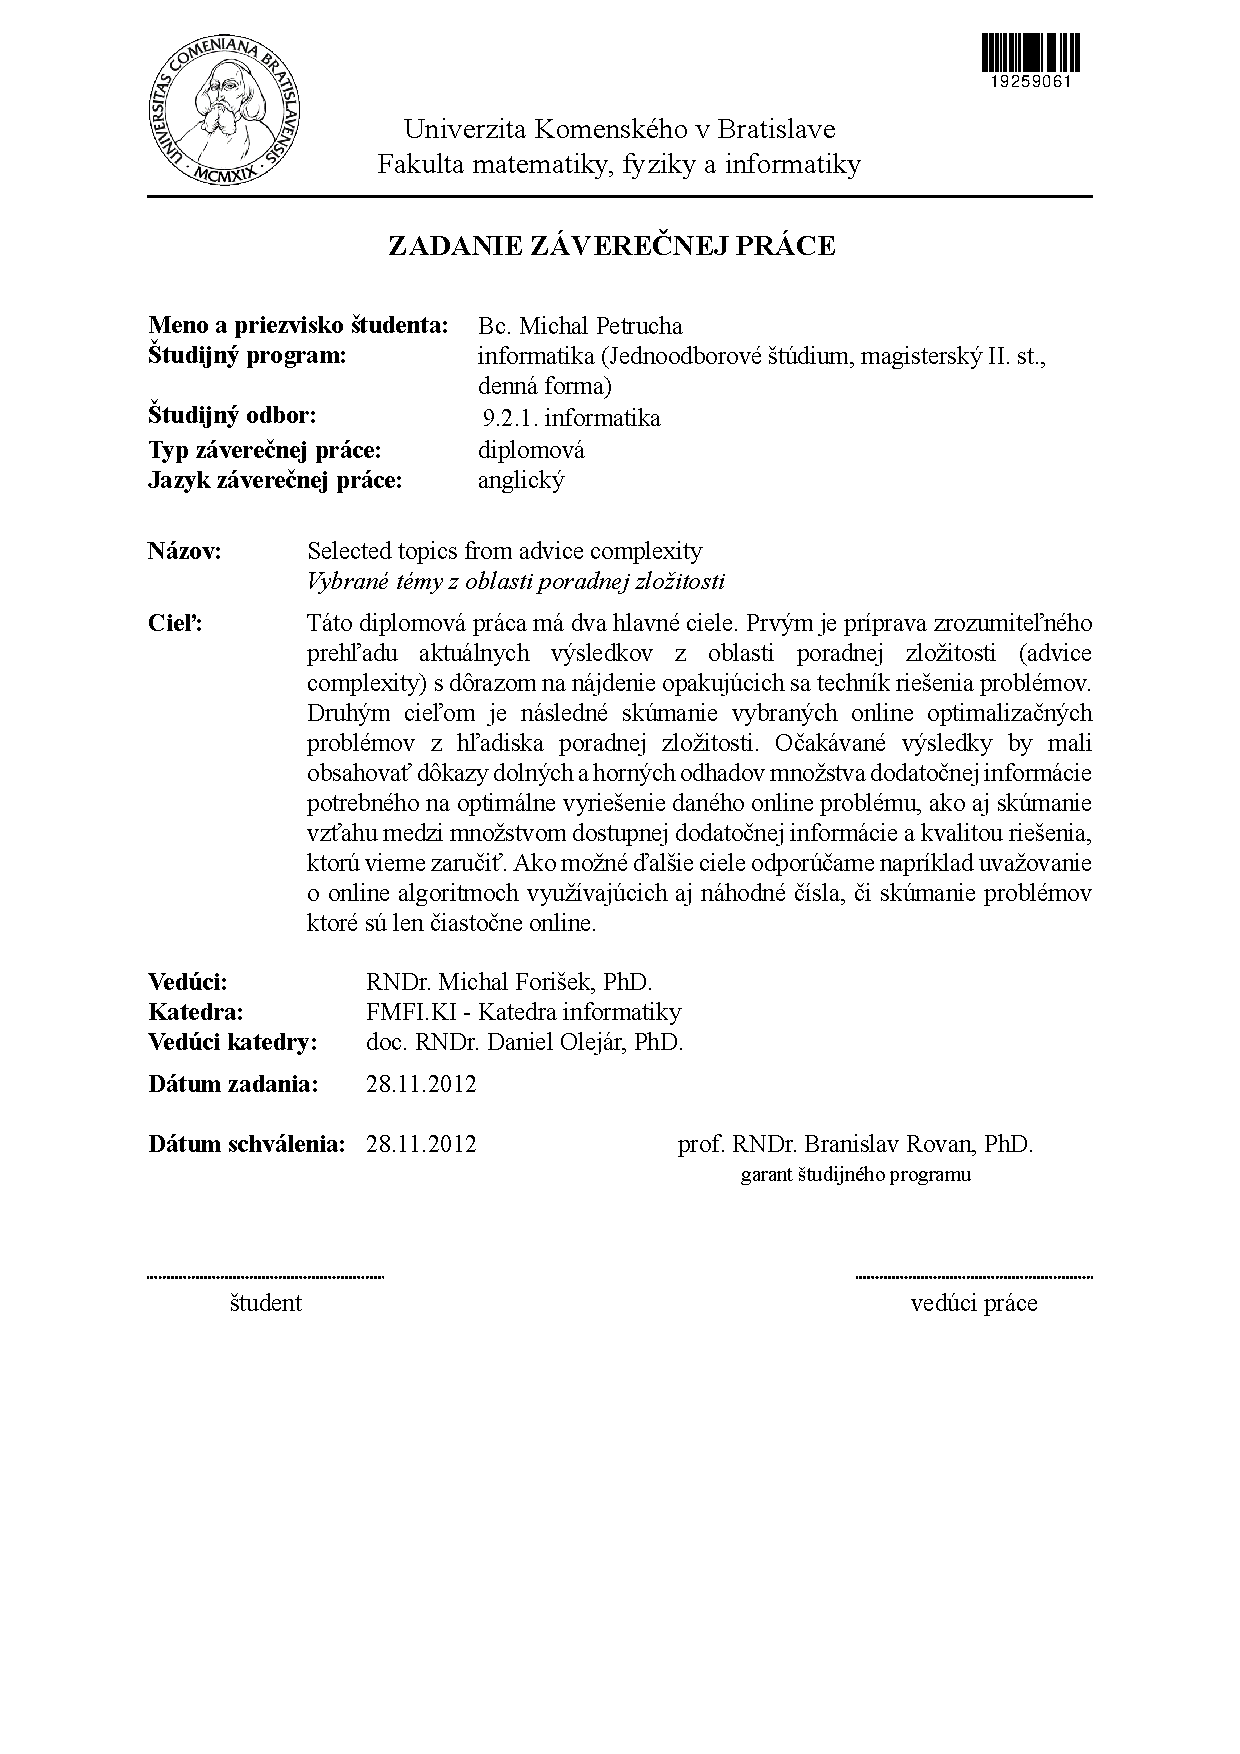
\includepdf{img/zadanie.pdf}

\eject

%\includepdf{img/statement.pdf}

\eject

%%%%%%%%%%%%%%%%%% Abstrakty a poďakovanie %%%%%%%%%%%%%%%%%%
%\thispagestyle{empty}
\section*{Abstrakt}
Sem patrí abstrakt v~slovenčine.

\medskip
{\bf Kľúčové slová:} nejaké sem treba doplniť



\eject

%\thispagestyle{empty}
\section*{Abstract}
This is where the abstract in English will go.

\medskip
{\bf Key words:} and some key words as well



\eject

\section*{Acknowledgements}
I want to thank Valve for their Holiday sales on Steam which gave me a lot
of options to procrastinate instead of working on this thesis.


\eject

%\thispagestyle{empty}
\tableofcontents
%\thispagestyle{empty}

% S tymito dvomi sa este bude treba pohrat, hlavne aby nemali cislovane
% strany a vobec.
\listoffigures
\listoftables

\chapter*{Introduction}
\pagenumbering{arabic}
\setcounter{page}{1}
\addcontentsline{toc}{chapter}{Introduction}
\label{chapter:intro}
This is the place for an introduction\dots


\chapter{First chapter}
\label{chapter:first}

\todo{Write this introduction}
This is the sectionless introduction to the first chapter. Probably a word
or two about how we are going to give a brief overview of what online
problems and advice complexity are and the appropriate definitions upon
which this thesis is based.

\section{Online problems}
\label{section:online}
One of the countless ways to categorize algorithmic problems is into
\emph{offline} and \emph{online problems}. Offline problems are those
where the algorithm can access the whole input instance before yielding
the output.  On the other hand, the instance of an online problem is
revealed to the algorithm in smaller pieces and after each piece a partial
solution has to be produced. This partial solution cannot be changed
later.

A slightly different way of looking at online algorithms is that the
algorithm waits for an input query, processes it and outputs an answer to
this query immediately. Then it waits for another query and repeats the
process until there is nothing more to do.

Solving a problem online is obviously more difficult than solving the same
instance knowing the whole input at once. For many problems it is even
impossible to compute the optimal partial solutions without the knowledge
of the rest of the input sequence. Therefore we define a \emph{competitive
ratio} of an algorithm, which is the quotient of the cost of the solution
produced by the online algorithm and the cost of the optimal solution. An
optimal solution is one produced by an optimal offline algorithm. Since
the competitive ratio can depend on the input instance, we study the
worst-case competitive ratio an algorithm achieves.

We may consider randomized online algorithms as well. In this case we
examine the expected competitive ratio.

Let us describe a few examples of simple online problems to give a better
idea of what they are about. A very simple online problem is ski rental.
Suppose we are going to take an unknown number of ski trips and we do not
own a pair of skis. Renting a pair of skis for a single trip costs $1$,
buying one costs $s$. The input consists of a sequence of queries ``take a
ski trip'' and after each query an answer is expected that is either
``rent'', ``buy'' or ``use skis already bought''. In \cite{skirental} it
is proved that to minimize the competitive ratio the algorithm needs to
rent for the first $s-1$ rounds and then buy a pair of skis; this way, the
competitive ratio is $\frac{2s-1}{s} \approx 2$.

Another classic online problem is the paging problem. Assume a two-level
memory divided into uniform, fixed-size pages. Let $k$ be the number of
pages that can fit within the fast memory. The input consists of $n$
queries, each specifying a page we want to access. This page needs to be
loaded into the fast memory, thus replacing a page called a victim (unless
it is there already). The goal is to minimize the number of page faults,
i.e. the number of times we need to load a page from the slow memory into
the fast level.

In \cite{paging-deterministic} the authors show that for any deterministic
online algorithm solving the paging problem it is possible to construct an
instance using $k + 1$ pages where the online algorithm will produce a
page fault on each request by always choosing the page that is not in the
fast memory. However, an offline algorithm can decrease the number of page
faults by at least a factor of $k$, therefore the competitive ratio of any
online paging algorithm is at least $k$.

In addition, in \cite{paging-randomized} the authors describe a randomized
online algorithm for the paging problem whose competitive ratio is $H_k$.

\section{Advice complexity}
\label{section:advice}
In the previous section we showed that there are problems which cannot be
solved optimally by a deterministic online algorithm. This means that
having access to the whole of the input sequence can help the algorithm to
provide better partial results. However, sometimes it may not be necessary
to access the whole input sequence in order to compute the optimal
solution, in some cases a significantly smaller amount of information is
required.

That is why a computational model of \emph{online algorithms with advice}
has been introduced in \cite{advice-first}. In this model, the online
algorithm is assisted by an oracle with access to the entire input
sequence. The oracle has unlimited computational power and provides the
online algorithm with information about the input sequence that it
requires. We define the \emph{advice complexity} of an online algorithm as
the minimal number of bits it needs to read from the oracle in order to
solve the problem optimally. The advice complexity of an online problem is
then defined as the lowest advice complexity of online algorithms solving
it.

There have been multiple formal definitions of this model with various
drawbacks. \cite{advice-first} contains a definition in which the online
algorithm has access to a finite binary advice tape. That means, however,
that additional information can be encoded into the length of the advice
tape. In \cite{advice-constant} the authors define a slightly different
model where the online algorithm receives the same amount of information
in each round. This makes it impossible to use a sublinear amount of
advice. The model used in this thesis has been defined in
\cite{advice-infinite}; this model uses an infinite advice tape and we
measure the number of bits the algorithm accesses.

To illustrate the power of advice, we show the amount of advice required
to solve the two aforementioned online problems optimally. The ski rental
problem is trivial to solve using a single bit of advice -- this bit tells
the algorithm whether there will be at least $s$ queries. The online
algorithm reads this before answering the first query and it knows
immediately whether to buy a pair of skis or just rent them on each trip.

The paging problem is slightly more complex to solve optimally using
advice. Following the proof in \cite{paging-optimal}, this can be done
using $n$ bits of advice. The oracle calculates one optimal solution to
the input instance and assigns a single bit to each request. This bit
indicates whether the page will be accessed again before it is replaced by
another one in the optimal solution, such pages are called active; if the
page will not be accessed again, it is passive. The online algorithm then
just picks a passive page as the victim on each page fault.

Thus far we only covered the amount of advice required to obtain the
optimal solution using an online algorithm. However, it is also useful to
examine the amount of advice required to achieve a certain competitive
ratio and the tradeoff between these two. In this thesis we will study
this aspect as well.

Another possible area of research is the amount of advice required to
solve a \emph{partially online problem}. This is a special case of an
online problem where only a part of the input instance is served in pieces
and at some point the whole rest of the input is served in a single piece.

Taking the previous notion one step further, it also makes sense to apply
the concept of advice to offline problems. In that case, we no longer
study the competitive ratio. Instead, we can use advice to help an
algorithm achieve better efficiency, mainly in terms of its time
complexity, especially for known hard problems, such as $NP$-complete
problems. This direction of research is explored further in the last
chapter of this thesis.


\chapter*{Conclusion}
\addcontentsline{toc}{chapter}{Conclusion}
\label{chapter:conclusion}
Once the rest of the thesis is written, this is the place where a witty
conclusion will appear.


%\backmatter fixme: preco to tu nefunguje? asi chyba nejaky package

\printbibliography

\appendix

%\chapter{Implementation}
%\input{tex/50implementation.tex}

\end{document}
